%&../settings/preamble.main

\ifsubfile
\pagestyle{plain}
\setcounter{chapter}{15}

% arara: pdflatex: { options: ["--output-directory=../build"], draft: yes, synctex: no }
% arara: pdflatex: { options: ["--output-directory=../build"], synctex: no }
\begin{document}
\fi
\chapter{Backtrack}

\paragraph{Problemi tipici}
Problemi tipici sono:
\begin{itemize}
	\item \emph{elencare tutte le possibili soluzioni} (enumerazione), come ad esempio elencare tutte le possibili permutazioni di un insieme;
	\item \emph{costruire almeno una soluzione del problema}, in questo caso si utilizza l'algoritmo di enumerazione fermandosi alla prima soluzione dispoonibile;
	\item \emph{contare le soluzioni}, in alcuni casi è possibile contare in modo analitico, in altri casi si costruiscoo le soluzioni e si contano;
	\item \emph{trovare le soluzioni ottimali}, si enumerano tutte le soluzioni che vengono valutate tramite una funzione di costo.
	 	In questo caso si utilizzano anche altre tecniche di programmazione (come la programmazione dinamica, o la tecnica greedy).
\end{itemize}

\section{Eumerazione}

Per costruire tutte le soluzioni, si utilizza un approccio di \enquote{forza bruta} (\emph{brute force}).
In alcuni casi è l'unica strada percorribile.
Fortunatamente i processori moderni rendono affrontabili problemi considerati di dimensioni medio-piccole.
Inoltre, a volte lo spazio delle soluzioni non deve essere analizzato interamente.

\begin{idea}[backtracking]
\enquote{Prova a fare qualcosa, e se non va bene, disfalo e prova qualcos'altro}
\end{idea}

Il backtracking è una tecnica algoritmica che, come altre, deve essere personalizzata per ogni applicazione individuale.
Dobbiamo quindi trovare un metodo sistematico per iterare su tutte le possibili istanze di uno spazio di ricerca.

\paragraph{Organizzazione del problema}
Una soluzione viene rappresentata come il vettore \(S[1][n]\);
il contenuto degli elementi \(S[i]\) è una \emph{sequenza di scelte} (possibili) \(C\) dipendenti dal problema.

Ad esempio preso un insieme \(C\) che rappresenta un insieme generico possiamo avere possibili \emph{permutazioni} o \emph{sottoinsiemi}.
Se \(C\) è un insieme di mosse ottenerremo una \emph{sequenza di mosse};
se nell'insieme \(C\) sono contenuti archi di un grafo, allora otterremo possibili percorsi del grafo; e così via.

\paragraph{Scherma di risoluzione generale}
Ad ogni passo, partiamo da una soluzione generale \(S[1][k]\) in cui \(k \geqslant 0\) scelte sono state prese (ovvero abbiamo effettuato \(k\) scelte, dove \(k\) può essere anche nullo).

Se la sequenza di scelte che abbiamo effettuato (\(S[1][k]\)) costituiscono una soluzione ammissibile allora la \enquote{processiamo}.
Può essere quindi stampata, contata, valutata, oppure si può decidere di terminare elencando tutte le possibili soluzioni.

Indipendentemente dalla precedente se \(S[1][k]\) non rappresenta una soluzione completa, allora proviamo, se è possibile, ad \emph{estendere} \(S[1][k]\) con una delle possibili scelte in una soluzione \(S[1][k+1]\);
altrimenti \enquote{cancelliamo} l'ultima scelta effettuata \(S[k]\) tornando sui nostri passi (facendo quindi \emph{backtracking}) e ripartendo dalla soluzione precedente \(S[1][k-1]\).

\paragraph{Rappresentazione del problema}
Il nostro problema viene rappresentato da un \emph{albero di decisione} nel quale:
\begin{itemize}
	\item lo \emph{spazio di ricerca} viene rappresentato dall'albero stesso;
	\item la \emph{soluzione parziale vuota} (ossia quella dove non abbiamo preso nessuna decisione) è la radice;
	\item le \emph{soluzioni parziali} sono rappresentate dai nodi interni;
	\item le \emph{soluzioni ammissibili} vengono rappresentate dalle foglie.
\end{itemize}

\subparagraph{Pruning}
I \enquote{rami} dell'albero che sicuramente non portano a soluzioni ammissibili possono essere \enquote{potati} (\emph{pruned}).
La valutazione della \enquote{potatura} viene effettuata nelle soluzioni parziali radici del sottoalbero da potare.

\begin{note}
Il pruning riduce drasticamente lo spazio delle soluzioni del problema.
\end{note}

% TODO subfigure
\begin{figure}
\begin{subfigure}[t]{.6\textwidth}
	\begin{forest} compact tree
	[[[[[][]][[][]]][[[][]][[][]]]][[[[][]][[][]]][[[][]][[][]]]]]
	\end{forest}
	\caption{Lo spazio di ricerca di un determinato problema è rappresentato da un albero delle decisioni}%
	\label{fig:tree-backtrack}
\end{subfigure}
\begin{subfigure}[t]{.4\textwidth}\flushright
	\begin{forest} compact tree
	[[,pruned red
		[[[][]][[][]]][[[][]][[][]]]
	]
	[
		[[[][]][,pruned red
			[][]]
		]
		[,pruned red
			[[][]][[][]]]
		]
	]
	\end{forest}
	\caption{\emph{pruning} dei rami}%
	\label{fig:tree-backtrack-pruned}
\end{subfigure}
\caption{Un albero di decisione ed il suo corrispondente albero potato dei rami che non portano a soluzioni ammissibili.}
\end{figure}

\paragraph{Approcci}
Ci sono due possibili approcci alla tecnica del backtracking:
\begin{enumerate}
	\item la prima consiste nello sviluppo di un algoritmo \emph{ricorsivo} che lavora tramite una visita in profondità nell'albero delle scelte;
	\item la seconda consiste nello sviluppo di un algoritmo \emph{iterativo} ed utilizza un approccio ingordo (\foreign{greedy}), eventualmente tornando sui propri passi (effetuando quindi \foreign{backtracking}).
\end{enumerate}

Sia il problema dell'inviluppo convesso, che quello della corrispondenza fra stringhe (\emph{string matching}) utilizzano questo approccio.

In base alle \(i\) scelte già effettuate decido quali sono le mie future scelte.

\begin{algorithm}[H]
\caption{Schema generale per il problema dell'enumerazione}

\prototype{\Bool \enumeration{\Item{} S, \Int n, \Int i, \dots}}{
	\params{S}[vettore contenente le soluzioni parziali \(S[1][i]\)]
	\params{n}[il numero massimo di scelte possibili]
	\params{i}[indice corrente]
	\params{\dots}[parametri addizionali dipendenti dal problema]

	\BlankLine
	\BlankLine
	\Set \(C = \getChoices{S, n, i, \dots}\) \Comment*[h]{Determina \(C\) in funzione di \(S[1][i-1]\)}

	\params{C}[l'insieme dei possibili candidati per estendere la soluzione]

	\BlankLine
	\ForEach(\tcp*[h]{per ogni possibile scelta fra quelle possibili}){\(c \in C\)}{
		\(S[i] \Assign c\) \Comment*[l]{registro la scelta}

		\BlankLine
		\If{\(\isAdmissible{S, n, i}\)}{
			\tcp{\(S[1][i]\) è una soluzione ammissibile}
			\If{\(\processSolution{S, n, i, \dots}\)}{
				\tcp{vogliamo bloccare l'esecuzione alla prima soluzione possibile}
				\Return \True
			}
		}

		\BlankLine
		\tcp{non decido di fermarmi alla prima soluzione ammissibile}
		\If{\(\enumeration{S, n, \(\mhl{i+1}\), \dots}\)}{
			\tcp{effettuo la \(i+1\)-esima scelta}
			\Return \True
		}
	}
	\tcp{non ho trovato la soluzione cercata}
	\Return \False\;
}

\end{algorithm}

\newpage
\subsection{Problemi che trattano di sottoinsiemi}

\paragraph{Definizione del problema}
Elencare tutti i sottoinsiemi dell'insieme \(\{1, \dots, n\}\)

\begin{minipage}[t]{.5\linewidth}
	\begin{algorithm}[H]
	\caption{Primo tentativo}

	\prototype{\subSets{\Array{\Int} S, \Int n, \Int i}}{
		\Set \(C \Assign \iif{\(i \leqslant n, \{ 0,1 \}, \emptyset\)}\)

		\BlankLine
		\ForEach{\(c \in C\)}{
			\(S[i] \Assign c\)\;

			\BlankLine
			\If{\(i \Equal n\)}{
				\processSolution{S, n}\;
			}
			\subSets{\(S\), \(n\), \(i+1\)}\;
		}
	}

	\end{algorithm}
\end{minipage}
\begin{minipage}[t]{.5\linewidth}
	\begin{algorithm}[H]
	\caption{Versione \enquote{più pulita}}

	\prototype{\subSets{\Array{\Int} S, \Int n, \Int i}}{

		\BlankLine
		\ForEach{\(c \in \{0,1\}\)}{
			\(S[i] \Assign c\)\;

			\BlankLine
			\eIf{\(i \Equal n\)}{
				\processSolution{S, n}\;
			}{
				\subSets{\(S\), \(n\), \(i+1\)}\;
			}
		}
	}

	\end{algorithm}
\end{minipage}

Fare riferimento alla \href{https://youtu.be/00hO1skHCls?t=1420}{spiegazione grafica} qui non riportata.

\paragraph{Considerazioni}
Non c'è pruning.
Tutto lo spazio possibile viene esplorato.
Ma questo avviene per definizione.
Questo porta ad una complessità di \(\Omicron(n \cdot 2^n)\).
\`{E} possbile pensare ad una soluzione iterativa, ad-hoc? (che non utilizza la tecnica del backtracking)

\begin{algorithm}[H]
\caption{Versione \enquote{più pulita}}

\prototype{\subSets{\Array{\Int} S, \Int n, \Int i}}{

	\BlankLine
	\From(\Comment*[h]{\(\Omicron(n^2)\)}){\(j = 0\) \DownTo \(2^n - 1\)}{
		\Print \enquote{\{}

		\BlankLine
		\From(\Comment*[h]{\(\Omicron(n)\)}){\(i = 0\) \DownTo \(n-1\)}{
			\If{(\(j\) \And \(2^{i}) \neq 0\)}{
				\Print \(i\)\;
			}
			\Print \enquote{\}}
		}
	}
}

\end{algorithm}

\newpage
\paragraph{Definizione del problema}
Elencare tutti i sottoinsiemi di dimensione \(k\) di un insieme \(\{1, \dots, n\}\)

\begin{minipage}[t]{.5\linewidth}
	\begin{algorithm}[H]
	\caption{Tentativo 1}

	\prototype{\subSets{\Array{\Int} S, \Int n, \Int k, \Int i}}{

		\BlankLine
		\Set \(C \Assign \iif{\(i \leqslant n, \{ 0,1 \}, \emptyset\)}\)

		\BlankLine
		\ForEach{\(c \in C\)}{
			\(S[i] \Assign c\)\;

			\BlankLine
			\If{\(i \Equal n\)}{
				\Int \(count\) \Assign 0\;

				\BlankLine
				\From{\(j \Assign 1\) \DownTo \(n\)}{
					\AddTo{count}{S[j]}\;
				}

				\BlankLine
				\If{\(count \Equal k\)}{
					\tcp{ho finito}
					\processSolution{S, n}\;
				}
			}
		}
		\subSets{S, n, k, i+1}\;
	}

	\end{algorithm}
\end{minipage}
\begin{minipage}[t]{.5\linewidth}
	\begin{algorithm}[H]
	\caption{Tentativo 2}

	\prototype{\subSets{\omitted, \Int count}}{

		\BlankLine
		\Set \(C \Assign \iif{\(i \leqslant n, \{ 0,1 \}, \emptyset\)}\)

		\BlankLine
		\ForEach{\(c \in C\)}{
			\(S[i] \Assign c\)\;
			\AddTo{count}{S[i]}\;

			\BlankLine
			\tcp{logica dell'algoritmo}
			\If{\(i \Equal n\) \And \(count \Equal k\)}{
				\processSolution{S, n}\;
			}

			\subSets{S, n, k, i+1, count}\;
			\RemoveFrom{count}{S[i]}\;
		}
	}

	\end{algorithm}
	\vspace{-10pt}
	Tengo conto del contatore nelle chiamate successive e gli sottraggo i valori aggiunti nelle chiamate di \emph{backtracking}.
\end{minipage}

\begin{algorithm}[H]
\caption{Elencare tutti i sottoinsiemi di dimensione \(k\) di un insieme \(\{1, \dots, n\}\)}

\prototype{\subSets{\Array{\Int} S, \Int n, \Int k, \Int i, \Int count}}{
	\params{n}[numeri di elementi]
	\params{k}[numeri di elementi considerati]
	\params{i}[la scelta che ho già fatto]

	\BlankLine
	\tcp{se ho già raggiunto \(k\) o non ci sono abbastanza bit per arrivare a \(k\) non ho più bisogno di visitare il sotto-albero delle scelte relativo)}
	\Set \(C \Assign \iif{\(count < k\) \And \(count + (n-i+1) \geqslant k\), \(\{0,1\}\), \(\emptyset\)}\)\;
	\tcp{\(count < k\): ho ancora la possibilità di accendere un bit}
	\tcp{\(count + (n-i+1) \geqslant k\): ho ancora abbastanza bit da accendere per raggiungere \(k\)}

	\BlankLine
	\ForEach{\(c \in C\)}{
		\(S[i] \Assign c\)\;
		\tcp{i bit scelti non cambiano nelle chiamate successive}
		\AddTo{count}{S[i]} \Comment*[l]{sommo i bit a \(1\)}

		\BlankLine
		\eIf{\(count \Equal k\)}{
			\processSolution{S, i}\;
		}{
			\subSets{S, n, k, i+1, count}\;
		}

		\BlankLine
		\tcp{quando effettuo il \emph{backtrack} devo tornare allo stato precedente}
		\RemoveFrom{count}{S[i]} \Comment*[l]{sottraggo i bit a 1}
	}
}

\end{algorithm}

\paragraph{Considerazioni}
Abbiamo imparato che \enquote{specializzando} l'algoritmo generico, possiamo ottenere una versione più efficiente.
Tuttavia abbiamo ottenuto solo un miglioramento parziale (verso \(\nicefrac{n}{2}\)).

\begin{note}
\`{E} difficile ottenere la stessa efficienza con un algoritmo iterativo.
\end{note}

\newpage
\section{Permutazioni}

\paragraph{Definizione del problema}
Stampa tutte le permutazioni di un insieme \(A\).
L'insieme dei candidati dipende dalla soluzione parziale \emph{corrente}.

\NoCaptionOfAlgo
\begin{algorithm}[H]
\caption[Stampa tutte le permutazioni di un insieme \(A\)]{}

\prototype{\permutations{\Set \(A\), \Int \(n\), \Item[] \(S\), \Int \(i\)}}{
	\params{A}[insieme dalla quale prendo gli oggetti]
	\params{n}[numero di permutazioni]

	\BlankLine
	\ForEach{\(c \in A\)}{
		\(S[i] \Assign c\) \Comment*[l]{scelgo l'oggetto}
		\(A.\setRemove{c}\) \Comment*[l]{lo tolgo dall'insieme}

		\BlankLine
		\eIf{\(A.\setEmpty\)}{
			\processSolution{S, n}\;
		}{
			\tcp{l'insieme \(A\) ha un elemento in meno}
			\permutations{\(A\), \(n\), \(S\), \(i+1\)}\;
		}

		\BlankLine
		\(A.\setInsert{c}\)\;
	}
}

\end{algorithm}

% \newpage
\section{Problema delle otto regine}

\begin{minipage}[c]{.675\textwidth}
\paragraph{Definizione del problema}
Il problema consiste nello posizionare \(n\) regine in una scacchiera \(n \times n\), in modo tale che nessuna regina ne \enquote{minacci} un'altra.

\begin{idea}
Ogni riga ed ogni colonna deve contenere esattamente una regina.
\end{idea}

Rappresentiamo la scacchiera con un vettore \(S[1][n]\), effettuiamo \emph{pruning} eliminando le diagonali.

Il numero di soluzioni ammonta a \(n! = 8! = \num{40320}\) della quale solo \num{15720} vengono esplorate.
\end{minipage}\hfill
\begin{minipage}[c]{.3\textwidth}
	\centering
	% \begin{figure}[H]
		% \centering
		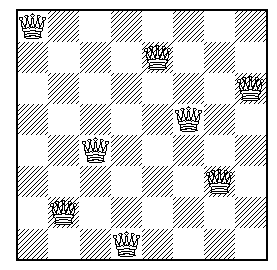
\includegraphics{chessboard-queens}
	% 	\caption{Soluzione del problema nel caso \(n=8\)}
	% 	\label{fig:chess-board}
	% \end{figure}
\end{minipage}

Esiste un algoritmo \emph{probabilistico} che risolve il problema in tempo lineare, tuttavia non garantisce che la terminazione sia sempre corretta.
Quindi viene fatto eseguire più volte fintanto che restituisce una soluzione corretta.
Il meccanismo consiste nel partire da una soluzione \enquote{ragionevolmente buona} e di muovere il pezzo con il più grande numero di conflitti nella posizione, all'interno della stessa colonna, in cui ne genera il numero minore.
La soluzione iniziale è scelta in modo \enquote{casuale} (ne parleremo più approfonditamente nel prossimo capitolo).
L'algoritmo si ferma quando non ci sono più pezzi da muovere.

\newpage
\section{Giro di cavallo}

\begin{minipage}{.675\textwidth}
\paragraph{Definizione del problema}
Lo scopo è trovare un \enquote{giro di cavallo}, ovvero un percorso di mosse valide del cavallo in modo che ogni casella venga visitata al più una volta.
\end{minipage}
\begin{minipage}{.3\textwidth}
	\centering
	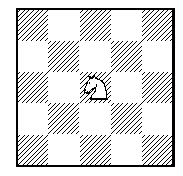
\includegraphics{chessboard-knight}
\end{minipage}

\subsection{Algoritmo risolutivo}

\begin{algorithm}[H]
\caption{Problema del giro di cavallo}

\prototype{\horse{\Matrix{\Int} \(S\), \Int \(i\), \Int \(x\), \Int \(y\)}}{

	\BlankLine
	\Set \(C \Assign \moves{S,x,y}\)\;

	\BlankLine
	\ForEach{\(c \in C\)}{
		\(S[x,y] \Assign i\) \Comment*[l]{ho raggiunto la posizione \((x,y)\) all'\(i\)-esimo passo}

		\BlankLine
		\uIf{\(i \Equal 64\)}{
			\processSolution{S}\;

			\BlankLine
			\Return \True\;
		}
		\ElseIf{\horse{\(S\), \(i+1\), \(x + m_{x}[c]\), \(y + m_{y}[c]\)}}{
			\tcp{effettuo l'\(i\)-esima mossa}

			\BlankLine
			\Return \True\;
		}

		\BlankLine
		\(S[x,y] \Assign 0\)
	}

	\BlankLine
	\Return \False
}

\BlankLine
\tcp{trova le possibili mosse}
\prototype{\moves{\Matrix{\Int} \(S\), \Int \(x\), \Int \(y\)}}{

	\BlankLine
	\Set \(C \Assign \setConstructor\)\;

	\BlankLine
	\tcp{fra tutte le possibili mosse}
	\From{\(i \Assign 1\) \DownTo \(8\)}{
		\tcp{calcola la nuova posizione}
		\(n_x \Assign x + m_x[i]\)\;
		\(n_y \Assign y + m_y[i]\)\;

		\BlankLine
		\If{\(1 \leqslant n_x \leqslant 8\) \And \(1 \leqslant n_y \leqslant 8\) \And \(S[n_x, n_y] \Assign 0\)}{

			\BlankLine
			\tcp{la posizione è libera}
			\(C\).\setInsert{i}\;
		}
	}

	\BlankLine
	\Return \(C\)
}

\end{algorithm}

Le prime due condizioni (\(1 \leqslant n_x \leqslant 8\) \And \(1 \leqslant n_y \leqslant 8\) controllano se rientro nei limiti della scacchiera, mentre la terza (\(S[n_x, n_y] \Assign 0\)) controlla se la posizione non è stata toccata.

% \paragraph{Complessità}

\newpage
\section{Sudoku}

\begin{figure}[H]
	\centering
	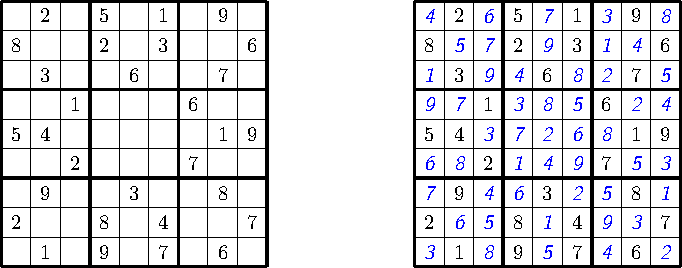
\includegraphics{sudoku}
	\caption{Il gioco del sudoku}
	\label{fig:sudoku}
\end{figure}

\subsection{Algoritmo risolutivo}

\begin{minipage}[t]{.5\textwidth}
	\begin{algorithm}[H]
	\caption{Sudoku}

	\prototype{\Bool \sudoku{\Matrix{\Int} S, \Int i}}{

		\BlankLine
		\Int \(x \Assign i \bmod 9\)\;
		\Int \(y \Assign \lfloor i / 9 \rfloor\)\;
		\Set \(C \Assign \setConstructor\)\;

		\BlankLine
		\tcp{il numero è già stato scelto}
		\eIf{\(S[x,y] \neq 0\)}{
			\(S\).\setInsert{\(S[x,y]\)}\;
		}{
			\tcp{inseriamo un numero}
			\From{\(c \Assign 1\) \DownTo \(9\)}{
				\If{\check{\(S\), \(x\), \(y\), \(c\)}}{
					\(C\).\setInsert{c}\;
				}
			}
		}

		\BlankLine
		\Int \(old \Assign S[x,y]\)\;
		\ForEach{\(c \in C\)}{
			\(S[x,y] \Assign c\)\;

			\BlankLine
			\tcp{arriviamo all'ultima casella}
			\If{\(i \Equal 80\)}{
				\processSolution{S,n}\;
				\Return \True
			}

			\BlankLine
			\If{\(\sudoku{\(S\), \(i+1\)}\)}{
				\Return \True
			}
		}

		\BlankLine
		\(S[x,y] \Assign old\)\;
		\Return \False
	}
\end{algorithm}
\end{minipage}%
\begin{minipage}[t]{.55\textwidth}
\begin{algorithm}[H]
\caption*{}

\tcp{se posso inserire un numero in quella cella}
\prototype{\check{\Matrix{\Int} \(S\), \Int \(x\), \Int \(y\), \Int \(c\)}}{

	\BlankLine
	\From{\(j \Assign 0\) \DownTo \(8\)}{
		\tcp{controllo sulla colonna}
		\If{\(S[x,j] \Equal c\)}{
			\Return \False
		}

		\BlankLine
		\tcp{controllo sulla riga}
		\If{\(S[j,y] \Equal c\)}{
			\Return \False
		}
	}

	\BlankLine
	\Int \(b_x \Assign \floor{x/3}\)\;
	\Int \(b_y \Assign \floor{y/3}\)\;
	\From{\(i_x \Assign 0\) \DownTo \(2\)}{
		\From{\(i_y \Assign 0\) \DownTo \(2\)}{
			\tcp{controllo sottotabella}
			\If{\(S[b_x \cdot 3 + i_x, b_y \cdot 3 + i_y] = c\)}{
				\Return \False
			}
		}
	}
}

% TODO mette le minipage all'interno
% NOTE lunghezza totalmente arbitraria
\vspace{104.6pt}
\end{algorithm}
\end{minipage}

\newpage
\section{Inviluppo convesso}

\begin{definition}[poligono convesso]
Un poligono nel piano è \alert{convesso} se ogni segmento di retta che congiunge due punti del poligono sta interamente nel poligono stesso, incluso il bordo.
\end{definition}

\paragraph{Definizione del problema}
Dati \(n\) punti \(p_1, \dots, p_n\) nel piano, con \(n \geqslant 3\), l'\alert{inviluppo convesso} (\emph{convex null}) è il più piccolo poligono convesso che li contiene tutti.

\subsection{Algoritmo inefficiente}

Un poligono può essere rappresentato per mezzo dei suoi spigoli.
Si consideri la retta che passa per una coppia di punti \((p_i, p_j)\), che divide il piano in due semipiani chiusi.
Se tutti i rimanenti \(n-2\) punti stanno dalla \emph{stessa parte}, allora lo spigolo \(S_{ij}\) fa parte dell'inviluppo convesso.

\NoCaptionOfAlgo
\begin{algorithm}[H]
\caption[]{inserire didascalia}

Data una retta definita dai punti \(p_1\) e \(p_2\), determinare se due punti \(p\) e \(q\) stanno nello stesso semipiano definito dalla retta.

\begin{figure}[H]
	\centering
	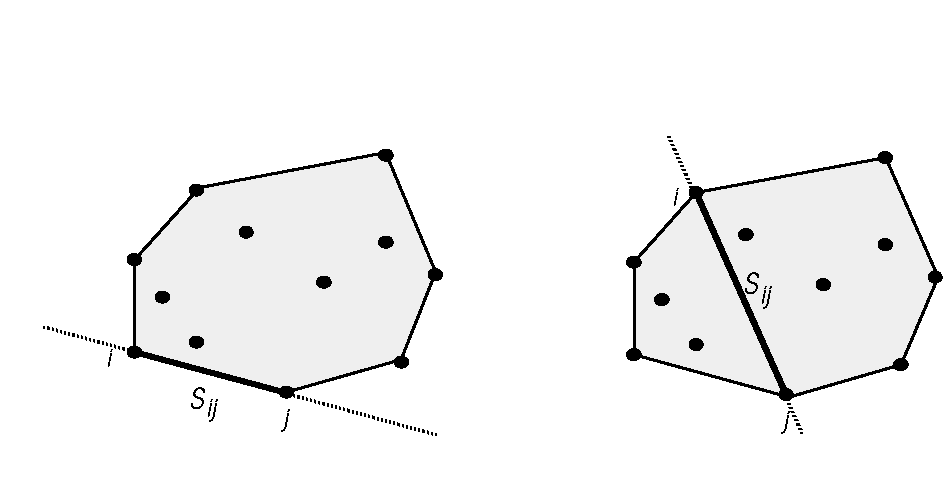
\includegraphics[scale=.5]{16-back-geometry2}
\end{figure}

\prototype{\Bool \stessaparte{\Point \(p_1\), \Point \(p_2\), \Point \(p\), \Point \(q\)}}{
	\Real \(dx \Assign p_2.x - p_1.x\)\;
	\Real \(dy \Assign p_2.y - p_1.y\)\;
	\Real \(dx_1 \Assign p.x - p_1.x\)\;
	\Real \(dy_1 \Assign p.y - p_1.y\)\;
	\Real \(dx_2 \Assign q.x - p_2.x\)\;
	\Real \(dy_2 \Assign q.y - p_2.y\)\;

	\BlankLine
	\tcp{se \(\geqslant 0\) allora sono dalla stessa parte}
	\Return \(((dx \cdot dy_1 - dy \cdot dx_1) \cdot (dx \cdot dy_2 - dy \cdot dx_2) \geqslant 0)\)\;
}

\end{algorithm}

% \begin{figure}[H]
% 	\centering
% 	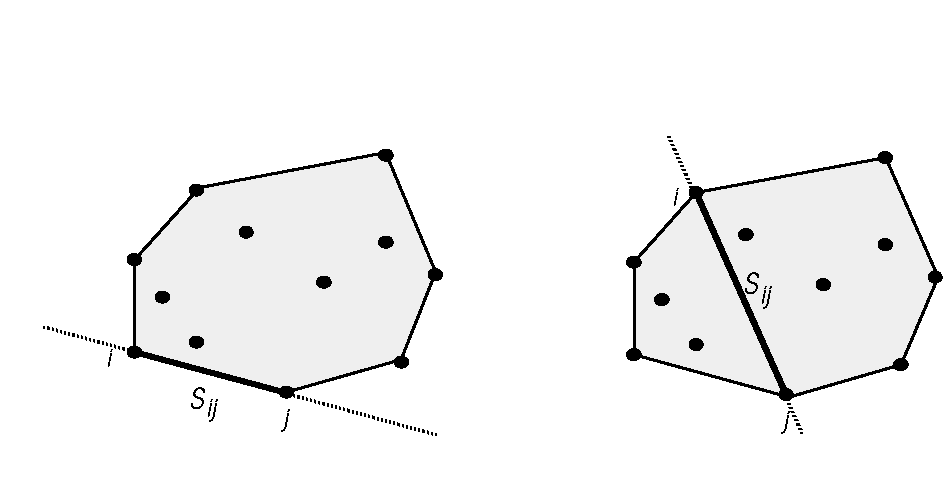
\includegraphics[scale=.5]{16-back-geometry2}
% 	% \caption{}
% 	% \label{fig:}
% \end{figure}

\paragraph{Complessità}
Prendiamo tutte le coppie di punti (\(n^2\)) e controlliamo se tutti gli altri punti (\(n-2\)) stanno \enquote{dall'altra parte}.
La complessità ammonta a \(\Omicron(n^2 \cdot (n-2) = \Omicron(n^3)\)

\newpage
\subsection{Algoritmo di Graham}

\begin{minipage}[c]{.5\linewidth}
	\paragraph{Prima fase}
	\begin{itemize}
		\item il punto con ordinata minima fa parte dell'inviluppo convesso;
		\item si ordinano i punti in base all'angolo formato dalla retta passante per il punto con ordinata minima e la retta orizzontale.
	\end{itemize}
\end{minipage}\hfill
\begin{minipage}[c]{.4\linewidth}
	\centering
	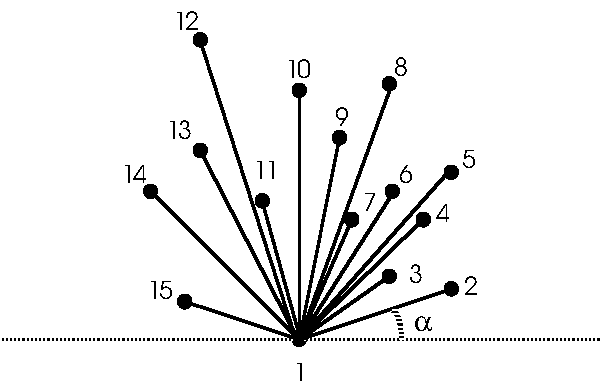
\includegraphics[scale=.5]{16-back-geometry3}
\end{minipage}

\begin{minipage}[c]{.5\linewidth}
	\paragraph{Seconda fase}
	\begin{itemize}
		\item inserisci \(p_1\), \(p_2\) nell'inviluppo corrente;
		\item per tutti i punti \(p_i = 3, \dots, n\):
		\begin{enumerate}
			\item siano \(p_h\) e \(p_j\), con \(h < j = i - 1\), gli ultimi due vertici dell'inviluppo corrente;
			\item scandisci a \enquote{ritroso} i punti nell'inviluppo \enquote{corrente} ed elimina \(p_j\) se \stessaparte{\(p_j\),\(p_h\),\(p_1\),\(p_i\)} \(\Equal\) \False;
			\item termina tale scansione se \(p_j\) non deve essere eliminato;
			\item aggiungi \(p_i\) all'inviluppo \enquote{corrente}.
		\end{enumerate}
	\end{itemize}
\end{minipage}\hfill
\begin{minipage}[c]{.4\linewidth}
	\centering
	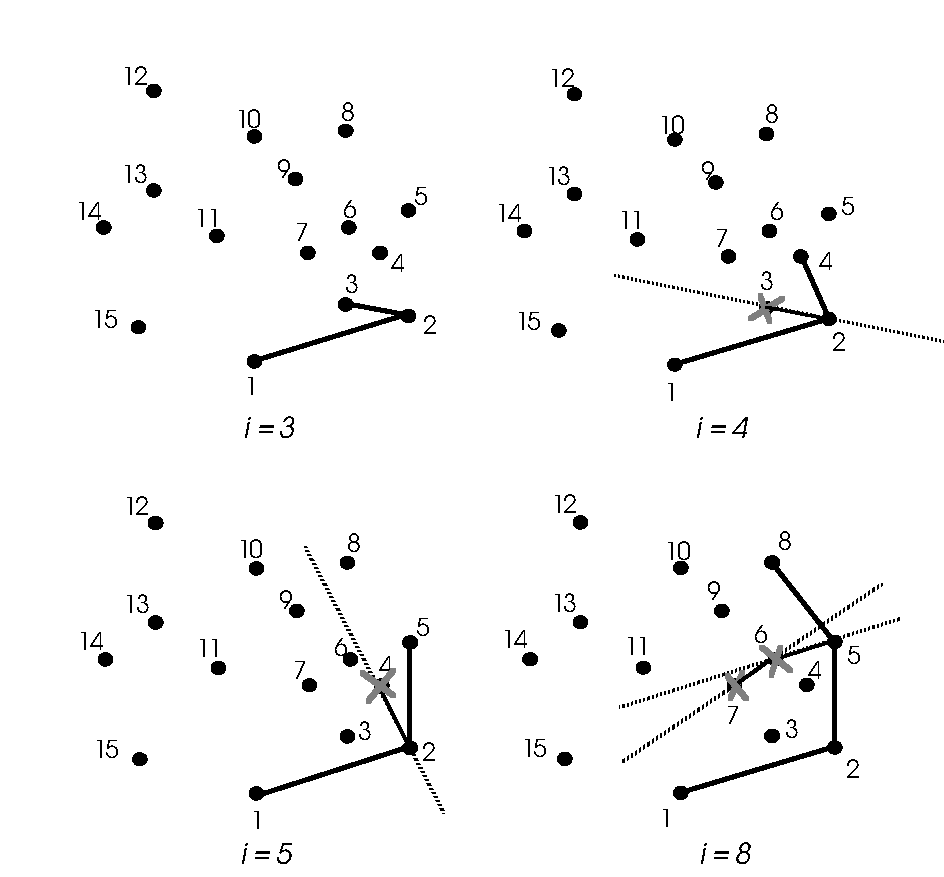
\includegraphics[scale=.5]{16-back-geometry4}
\end{minipage}

\begin{algorithm}[H]
\caption{Algoritmo di Graham}

\prototype{\Stack \graham{\Point p, \Int n}}{

	\BlankLine
	\Int \(min = 1\)\;

	\BlankLine
	\tcp{trovo il minimo}
	\From{\(i \Assign 2\) \DownTo \(n\)}{
		\If{\(p[i].y < p[min].y\)}{
			\(min \Assign i\)\;
		}
	}

	\BlankLine
	\Swap{\(p[1]\)}{\(p[min]\)}\;

	\BlankLine
	\{ riordina \(p[2, \dots, n]\) in base all'angolo formato rispetto all'asse orizzontale quando sono connessi con \(p[1]\)\}\;

	\BlankLine
	\{ elimina eventuali punti \enquote{allineati} tranne i più lontani da \(p_1\), aggiornando \(n\) \}

	\BlankLine
	\Stack \(S \Assign \stackConstructor\)\;
	\tcp{inserisci \(p_1\), \(p_2\) nell'inviluppo corrente}
	\(S\).\stackPush{\(p_1\)}\;
	\(S\).\stackPush{\(p_2\)}\;

	\BlankLine
	\tcp{per tutti gli altri punti}
	\From{\(i \Assign 3\) \DownTo \(n\)}{

		\BlankLine
		\tcp{escludo tutti i punti all'interno dell'inviluppo}
		\While(\tcp*[h]{\stackTopDue restituisce il secondo elemento}){\Not \stessaparte{S.\stackTop, S.\stackTopDue, \(p_1\), \(p_i\)}}{
			\(S\).\stackPop\;
		}

		\(S\).\stackPush{\(p_i\)}\;
	}
}

\begin{comment}
\BlankLine
\prototype{\Bool \stessaparte{\Point \(p_1\), \Point \(p_2\), \Point \(p\), \Point \(q\)}}{
	\Real \(dx = p_2.x - p_1.x\)\;
	\Real \(dy = p_2.y - p_1.y\)\;
	\Real \(dx_1 = p.x - p_1.x\)\;
	\Real \(dy_1 = p.y - p_1.y\)\;
	\Real \(dx_2 = q.x - p_2.x\)\;
	\Real \(dy_2 = q.y - p_2.y\)\;

	\BlankLine
	\Return \(((dx \cdot dy_1 - dy \cdot dx_1) \cdot (dx \cdot dy_2 - dy \cdot dx_2) \geqslant 0)\)\;
}
\end{comment}

\end{algorithm}

\vspace{-.5cm}
\paragraph{Complessità}
L'algoritmo di Graham ha complessità \(\Omicron(n \log n)\) in quanto è dominato dall'ordinamento dei punti.

\ifsubfile
\end{document}
\fi
